\documentclass[10pt]{article}
\usepackage[a4paper,margin=18mm]{geometry}
\usepackage{amsmath,amssymb,graphicx,hyperref}
\hypersetup{colorlinks=true,urlcolor=blue}
\setlength{\parindent}{0pt}\setlength{\parskip}{6pt}
\begin{document}
\begin{center}\Large A many-coset torus base\\[3pt]
\normalsize Conditional algebra and native membership, 16 November 2026\\
All PCC standing unverified\end{center}

\textbf{Construction.} Put $a=60824497$, $q=213156431$,
$M=aq=12965132697890207$, $k=20633$. In a field, assume
$h$ has exact order $M$. Set
\[
 S=\{h^{j+at}:1\le j\le k,\ 0\le t<q\}.
\]
The fixed index map is injective, so $|S|=kq=4398056640823$.
It excludes one and inverse pairs: any inverse collision would force
$a\mid j+j'$, while $0<j+j'\le2k<a$.
Every element is an $M$th root; odd $M$ excludes sign and negative-inverse
pairs in characteristic other than two. Existing Mathlib laws supply these
conditional endpoints. PCC-20261116-ac25ef. [pcc:unverified]

\begin{center}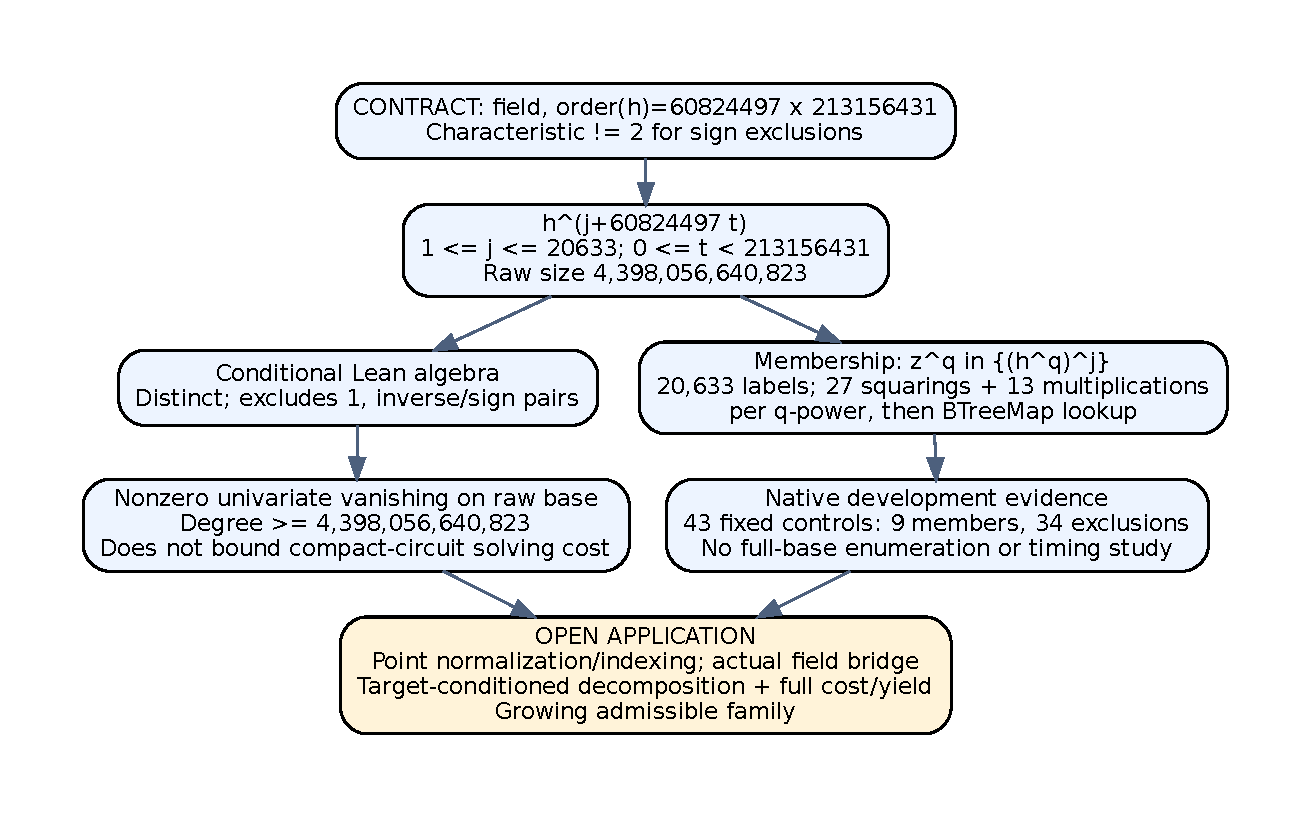
\includegraphics[width=0.98\linewidth,height=112mm,keepaspectratio]{pipeline.pdf}\end{center}

This is a raw-coordinate construction. Lean assumes the actual field/order
instance. The native control reuses the earlier exact-order/norm-one
parameter checker. Elligator/cofactor normalization, point indexing,
target-conditioned decomposition and an admissible growing family remain
open contracts. No novel coset principle is asserted.

\newpage
\begin{center}\Large Recognition cost and its boundary\end{center}

\textbf{Complete membership characterization.}
\[
 z\in S\quad\Longleftrightarrow\quad
 z^q\in\{(h^q)^j:1\le j\le k\}.
\]
For the converse, $(z/h^j)^q=1$; Mathlib's primitive-root enumeration
expresses it as $(h^a)^t$, $t<q$. Candidates need not be promised members
of the parent subgroup. PCC-20261116-ac25ef. [pcc:unverified]

\textbf{Implemented work.} Given $h$, one $q$th power and 20632 additional
Fp2 multiplications build 20633 labels. Each query computes a $q$th power
with 27 squarings and 13 multiplications using the existing implementation,
then performs a BTreeMap lookup on both canonical Fp coordinates, with
$O(\log k)$ comparisons and $O(k)$ stored labels. Parameter generation and
checks, allocation, conversion and indexing are additional costs.
Recognition returns $j$, not the subgroup exponent $t$ or an elliptic-point
matrix index. No performance price was measured. PCC-20261116-cc48bc.
[pcc:unverified]

\textbf{Native evidence.} 43 predetermined correctness cases cover 9 members
and 34 exclusions, including negative/inverse images, boundary exponents,
zero and an outside-parent generator. The example test, formatting and
strict Clippy pass. Pre-call source/binary digests, 33 matching source-input
hashes and a 51784-byte post-call archive retain the inputs. No base
enumeration, sampling, solver, paid job or broad root-library rerun occurred.
PCC-20261116-cc48bc. [pcc:unverified]

\textbf{Polynomial boundary.} Mathlib root counting applied to the same
injection gives, for every nonzero univariate $P$ vanishing on all of $S$,
\[
 \deg P\ge4398056640823.
\]
This excludes a smaller-degree raw-coordinate membership polynomial.
A dense coefficient array needs at least $|S|+1$ slots; this is not a
bound on sparse support, arithmetic-circuit size, changed coordinates,
multivariate solving degree or total attack work. Even linear dense input
cost alone does not disprove the proposed cost target.
PCC-20261116-1aecf2. [pcc:unverified]

\textbf{Next gate.} The native lookup is not a free polynomial-solver
primitive. Supply target-conditioned decomposition with original-ideal
witnesses, all coset constraints, setup, normalization/indexing, selection
and output work charged. In the earlier one-retained-row six-sum model at
$\beta=1/6$, an actual $\gamma<2$ is required to put its modeled exponent
below $1/2$; no such algorithm is supplied here. Multi-output methods retain
the separate query-aggregate contract. [pcc:unverified]

\textbf{Sources and reproduction.} Source-linked REPORT.md, Rust
\texttt{many\_coset\_audit.rs}, new Lean instance maps and raw control/gate
receipts. Mathlib at cfc55fc58714a59dc06e6e79edc6d1d95140d3c2;
\href{https://people.maths.ox.ac.uk/petit/files/16PKC_primeECDLP.pdf}{Petit--Kosters--Messeng,
PKC 2016, section 3.3} already supplies multiplicative-subgroup/coset bases.
Research-KB unavailable; pinned primary-source fallback used. Original route
criteria, frozen reports, source and evidence retain their bytes.
\end{document}
